\subsection{Experimental Methodology and Results}
In the following paragraphs, we report the methodology and results of our experiments.

\subsubsection{RQ1. Mono-objective SBSE Validation}
\paragraph{Method}
To answer the first research question RQ1, we implement three mono-objective search algorithms for compiler optimizations exploration (RS, GA and NS) in order to evaluate the non-functional properties of optimized code. We compare the performance results of different heuristics to standard GCC optimization levels (O1, O2, O3 and Ofast). 
In this experiment, we are trying to optimize for execution time (S), memory usage (MR) and CPU consumption (CR). Each non-functional property is improved separately and independently of other metrics. 

As it is shown on the left-hand side of figure 5, given a set of input programs \textit{"the training set"}, a list of optimizations and a performance objective, we use NOTICE to search for best optimization sequence. Thus, we generate a set of random Csmith programs \textit{"the training set"} (10 programs) and apply generated sequences to these programs. In this setting, the code quality metric is equal to the average performance improvement (S, MR or CR) and that, for all programs under test.




%the goal of this initial experiment is to: (1) evaluate the effectiveness of our component-based infrastructure to extract non-functional properties such as memory and CPU consumptions; (2) evaluate the performance of our proposed diversity-based exploration of optimization sequences (NS) to GA and RS; and finally (3) find the optimal solution relative to the input training set.

%The goal of this experiment is to show that NOTICE is able to generate 


\begin{figure}[h]
	\centering
	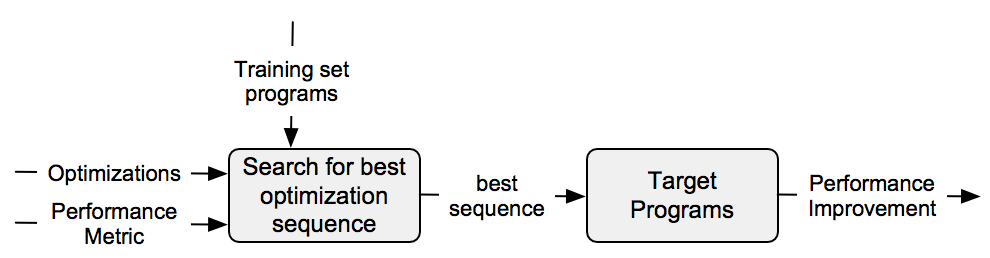
\includegraphics[width=1.\linewidth]{Ressources/sensitivity.png}
	\caption{fig}
\end{figure}


\paragraph{Results}
results



\begin{table}[h]
	\centering
	\caption{My caption}
	\label{my-label}
	\begin{tabular}{|l|l|l|l|l|l|l|c|}
		\hline
		& \textbf{O1}                    & \textbf{O2}                    & \textbf{O3}                    & \textbf{Ofast}                 & \textbf{RS}                    & \textbf{GA}                    & 
		\textbf{NS} \\
		\hhline{|=|=|=|=|=|=|=|=|}
		S  & \multicolumn{1}{c|}{} & \multicolumn{1}{c|}{} & \multicolumn{1}{c|}{} & \multicolumn{1}{c|}{} & \multicolumn{1}{c|}{} & \multicolumn{1}{c|}{} &    \\ \hline
		MR &                       &                       &                       &                       &                       &                       &    \\ \hline
		CR &                       &                       &                       &                       &                       &                       &    \\ \hline
	\end{tabular}
\end{table}
\

\noindent\fbox{\parbox{\linewidth-2\fboxrule-2\fboxsep}{
		\textbf{Key findings for RQ1.} \\
		blabla }}
\subsubsection{RQ2. Sensitivity}
\paragraph{Method}
Another interesting experiment is to test the sensitivity of \textit{"training set"} programs to compiler optimizations and evaluate the general applicability of best optimal optimization sets previously discovered in RQ1. To do so, we apply best discovered optimizations to new unseen Csmith (20 random programs) and Cbench programs (20 programs) and we compare then, the performance improvements (see right-hand side of figure 5). The idea of this experiment is to test whether only Csmith programs are more sensitive to compiler optimizations or not. If so, this will be useful for compiler users and researchers to use NOTICE in order to build general optimization sequences from their representative training set programs.

\paragraph{Results}
results

\noindent\fbox{\parbox{\linewidth-2\fboxrule-2\fboxsep}{
		\textbf{Key findings for RQ2.} \\
		blabla }}
\subsubsection{RQ3. Impact of optimizations on resource consumption}
\paragraph{Method}
To answer RQ3, we study the impact of standard optimization levels and best generated optimizations on memory and CPU consumption using NOTICE. Following again a mono-objective approach, we try in this experiment to maximize the speedup \textit{S} per-benchmark and study, at the same time, the impact of speedup \textit{S} on resource consumption namely memory footprint and CPU usage. 
In this experiment, we apply standard optimizations and different mono-objective heuristics individually to 5 Cbench programs and use NOTICE to profile applications in term of resource usage.   
The goal of this experiment is to: (1) use NOTICE infrastructure to provide an understanding of optimizations behavior, in term of resource consumption, when trying to optimize for execution time; (2) prove the usefulness of resource consumption reduction as a key objective for performance improvement.




\paragraph{Results}

%\begin{figure}[h]
%	\centering
%	\includegraphics[width=1.\linewidth]{Ressources/infra_novelty_stat2.png}
%	\caption{Evaluating the speedup after applying standard optimization options compared to best generated optimization using NS}
%\end{figure}
results

\noindent\fbox{\parbox{\linewidth-2\fboxrule-2\fboxsep}{
		\textbf{Key findings for RQ3.} \\
		blabla }}
\subsubsection{RQ4. Trade-offs between non-functional properties}
\paragraph{Method}

Finally, to answer RQ4, we use NOTICE to find trade-offs between non-functional properties. In this experiment, we choose to focus on the trade-off \textit{$<$ExecutionTime--MemoryUsage$>$}. We report the comparison results of our NS adaptation for optimizations generation to the current state-of-the-art multi-objective approaches namely NSGA-II and RS. 
  
Sequences evaluation is done across 5 Cbench programs as it is conducted in RQ1.
We evaluate the quality of the obtained Pareto optimal optimization levels, both qualitatively by visual inspection of the Pareto frontiers, and quantitatively by using the HV metric.

%Two tradeoffs are investigated in this section; $<$execution time--memory usage$>$ and $<$execution time--CPU usage$>$.


\paragraph{Results}
RESULTS

\noindent\fbox{\parbox{\linewidth-2\fboxrule-2\fboxsep}{
		\textbf{Key findings for RQ4.} \\
		blabla }}
\subsection{Discussions}
For RQ1, experiments take about 21 days to run all algorithms. These optimization times might seem long. However, it should be noted that this search can be conducted only once, since in RQ2, we show that best optimizations can be used with unseen programs of the same category as the training set, used to generate optimizations. This has to be proved with other case studies. As an alternative, it would be great to test model-based code generators. Code generators apply to same rules to generate new software programs. Thus, we can use NOTICE to define general-purpose optimizations from a set of generated code artifacts. 
Multi-objective search as conducted in RQ4, takes about 7 days, which we believe is acceptable for practical use. Nevertheless, speeding up the search speed
may be an interesting feature for future research.



%speeding up the search process may be an interesting avenue for future research.
\subsection{Threats to Validity}
Any automated approach has limitations. We resume, in the following paragraphs, external and internal threats that can be raised:
 
\textit{External validity} refers to the generalizability of our findings. In this study, we perform experiments on different widely used benchmark programs in iterative compilation. We also use to generate 30 Csmith programs (10 as training set and 20 for evaluation). However, we cannot assert that the best discovered set of optimizations can be generalized to industrial applications since optimizations are highly dependent on input programs and target architecture. In fact, experiments conducted on RQ1 and RQ2 have to be replicated to other case studies to confirm our findings; and build general optimization sequences from other representative training set programs chosen by compilers users.
Moreover, we build NOTICE to handle only optimizations performed by GCC versions, we did not investigate optimizations performed by other commonly used compilers, such as Clang or LLVM. In future work, we plan to provide more advanced version of NOTICE with multi-compiler evaluation.

\textit{Internal validity} is concerned with the causal relationship between the treatment and the outcome. Meta-heuristic algorithms are stochastic optimizers, they can provide different results for the same problem instance from one run to another. Are we providing a statistically sound method? or it is just a random result. Due to time constraints, we run all experiments only once. Following the state-of-art approaches in iterative compilation, previous works\cite{hoste2008cole,martinez2014multi} did not provide statistical tests to prove the effectiveness of their approaches. This is because experiments take too long time. However, we can deal with these internal threats to validity by performing at least 5 independent simulation runs for each problem instance.
 
 
\iffalse
\begin{table}[]
	\centering
	\caption{My caption}
	\label{my-label}
	\begin{tabular}{@{}|l|c|c|c|c|c|c|c|c|c|c|c|c|c|c|c|c|c|c|c|c|@{}}
		\toprule
		\multirow{2}{*}{} & \multicolumn{2}{c|}{CB1} & \multicolumn{2}{c|}{CB2} & \multicolumn{2}{c|}{CB3} & \multicolumn{2}{c|}{CB4} & \multicolumn{2}{c|}{CB5} & \multicolumn{2}{c|}{CS1} & \multicolumn{2}{c|}{CS2} & \multicolumn{2}{c|}{CS3} & \multicolumn{2}{c|}{CS4} & \multicolumn{2}{c|}{CS5} \\ \cmidrule(l){2-21} 
		& Ox & Best & Ox & Best & Ox & Best & Ox & Best & Ox & Best & Ox & Best & Ox & Best & Ox & Best & Ox & Best & Ox & Best \\ \midrule
		Execution Speedup & \begin{tabular}[c]{@{}c@{}}4\%\\ (O3)\end{tabular} &  &  &  &  &  &  &  &  &  &  &  &  &  &  &  &  &  &  &  \\ \midrule
		Memory & \begin{tabular}[c]{@{}c@{}}4\%\\ (O3)\end{tabular} &  &  &  &  &  &  &  &  &  &  &  &  &  &  &  &  &  &  &  \\ \midrule
		CPU & \begin{tabular}[c]{@{}c@{}}4\%\\ (O3)\end{tabular} &  &  &  &  &  &  &  &  &  &  &  &  &  &  &  &  &  &  &  \\ \midrule
		Compilation Speedup &  &  &  &  &  &  &  &  &  &  &  &  &  &  &  &  &  &  &  &  \\ \midrule
		Code Size &  &  &  &  &  &  &  &  &  &  &  &  &  &  &  &  &  &  &  &  \\ \bottomrule
	\end{tabular}
\end{table}
\fi


 

